\lab{Introduction to NumPy}{Introduction to NumPy}
\label{lab:NumPy}
\objective{NumPy is a powerful Python package for manipulating data with multi-dimensional vectors.
Its versatility and speed makes Python an ideal language for applied and computational mathematics.
\\ \indent
In this lab we introduce basic NumPy data structures and operations as a first step to numerical computing in Python.}

% More detailed / compelling objective?

\section*{Arrays} % ===========================================================

In many algorithms, data can be represented mathematically as a \emph{vector} or a \emph{matrix}.
Conceptually, a vector is just a list of numbers and a matrix is a two-dimensional list of numbers.
Therefore, we might try to represent a vector as a Python list and a matrix as a list of lists.
However, even basic linear algebra operations like matrix multiplication are cumbersome to implement and slow to execute when we store data this way.
The \emph{NumPy} module\footnote{NumPy is \emph{not} part of the standard library, but it is included in most Python distributions.} offers a much better solution.

The basic object in NumPy is the \emph{array}, which is conceptually similar to a matrix.
The NumPy array class is called \li{ndarray} (for ``$n$-dimensional array'').
The simplest way to explicitly create a 1-D \li{ndarray} is to define a list, then cast that list as an \li{ndarray} with NumPy's \li{array()} function.

\begin{lstlisting}
>>> import numpy as np
# Create a 1-D array by passing a list into NumPy's array() function.
>>> np.array([8, 4, 6, 0, 2])
array([8, 4, 6, 0, 2])
\end{lstlisting}
%
The alias ``\li{np}'' is standard in the Python community. % Make footnote?

An \li{ndarray} can have arbitrarily many dimensions.
A 2-D array is a 1-D array of 1-D arrays, and more generally, an $n$-dimensional array is a 1-D array of $(n-1)$-dimensional arrays.
Each dimension is called an \emph{axis}.
For a 2-D array, the 0-axis indexes the rows and the 1-axis indexes the columns.
Elements are accessed using brackets and indices (like a regular list), and the axes are separated by commas.

\begin{lstlisting}
# Create a 2-D array by passing a list of lists into array().
>>> A = np.array( [ [1, 2, 3],[4, 5, 6] ] )
>>> print(A)
[[1, 2, 3],
 [4, 5, 6]]

# Access elements of the array with brackets.
>>> print A[0, 1], A[1, 2]
2 6

# The elements of a 2-D array are 1-D arrays.
>>> A[0]
array([1, 2, 3])
\end{lstlisting}

\begin{problem} % Problem: Matrix Multiplication
NumPy's \li{dot()} function performs matrix multiplication. % In Python 3.5, we can use the @ operator to perform matrix multiplication.
Write a function that defines the following matrices as NumPy arrays.
\begin{align*}
A = \left[\begin{array}{rrr}
3 & -1 &  4 \\
1 &  5 & -9 \end{array}\right]
&&
B = \left[\begin{array}{cccc}
2 &  6 & -5 &  3\\
5 & -8 &  9 &  7\\
9 & -3 & -2 & -3\end{array}\right]
\end{align*}
Return the matrix product $AB$.
% Solution:
% array([[ 37,  14, -32, -10],
%        [-54,  -7,  58,  65]])

NumPy has excellent documentation.
For examples of array initialization and matrix multiplication, use IPython's object introspection feature to look up the documentation for \li{np.ndarray}, \li{np.array()} and \li{np.dot()}.
\begin{lstlisting}
In [1]: import numpy as np
In [2]: np.array?       # press 'Enter'
\end{lstlisting}
\label{prob:simple1}
\end{problem}

\subsection*{Basic Array Operations} % ----------------------------------------

NumPy arrays behave differently with respect to the binary arithmetic operators \li{+} and \li{*} than Python lists do.
For lists, \li{+} concatenates two lists and \li{*} replicates a list by a scalar amount (strings also behave this way).

\begin{lstlisting}
>>> x = [1, 2, 3]
>>> y = [4, 5, 6]

# Addition performs list concatenation.
>>> x + y
[1, 2, 3, 4, 5, 6]

# Mutliplication concatenates a list with itself a given number of times.
>>> x * 4
[1, 2, 3, 1, 2, 3, 1, 2, 3, 1, 2, 3]
\end{lstlisting}

In contrast, these operations are component-wise for NumPy arrays.
Thus arrays behave the same way that vectors and matrices behave mathematically.

\begin{lstlisting}
>>> x = np.array([1, 2, 3])
>>> y = np.array([4, 5, 6])

# Addition or multiplication by a scalar acts on each element of the array.
>>> x + 10
array([11, 12, 13])
>>> x * 4
array([ 4,  8, 12])

# Add two arrays together (component-wise).
>>> x + y
array([5, 7, 9])

# Multiply two arrays together (component-wise).
>>> x * y
array([ 4, 10, 18])
\end{lstlisting}

% Subtraction and division are also component-wise operations for NumPy arrays.
% Apart from being syntactically convenient, arithmetic operations on NumPy arrays also execute significantly faster than component-wise list operations.

\begin{comment} % Probably unnecessary.
\begin{warn} % Don't mix up * and np.dot().
Matrix multiplication is executed via \li{np.dot()} and scalar (component-wise) multiplication is executed via the \li{*} operator.
The equation below is an example of scalar multiplication, which uses \li{*}.
\begin{align*}
2 \left[\begin{array}{rrr}
1 & 2 & 3\\
4 & 5 & 6 \end{array}\right]
= \left[\begin{array}{rrr}
2 & 4 & 6\\
8 & 10 & 12 \end{array}\right]
\end{align*}
\end{warn}
\end{comment}

\begin{problem} % Problem: Simple Matrix Equation 2 (Cayley Hamilton)
Write a function that defines the following matrix as a NumPy array.
\[
A = \left[\begin{array}{rrr}
3 & 1 & 4\\
1 & 5 & 9 \\
-5 & 3 & 1 \end{array}\right]
\]
Return the matrix $-A^3 + 9A^2 - 15A$.

In this context, $A^2 = AA$ (the matrix product).
The somewhat surprising result is a demonstration of the Cayley-Hamilton theorem.
\label{prob:simple2}
\end{problem}

\subsection*{Array Attributes} % ----------------------------------------------
An \li{ndarray} object has several attributes, some of which are listed below.

\begin{table}[H] % Important ndarray Attributes
\centering
\begin{tabular}{c|l}
    Attribute & Description \\
    \hline \li{dtype} & The type of the elements in the array. \\
    \li{ndim} & The number of axes (dimensions) of the array. \\
    \li{shape} & A tuple of integers indicating the size in each dimension. \\
    \li{size} & The total number of elements in the array. \\
\end{tabular}
\end{table}

\begin{lstlisting}
>>> A = np.array([[1, 2, 3],[4, 5, 6]])
>>> A.ndim
2
>>> A.shape
(2, 3)
>>> A.size
6
\end{lstlisting}

Note that the \li{ndim} is the number of entries in \li{shape}, and the
the \li{size} of the array is the product of the entries of \li{shape}.

\begin{comment} % This is being severely shortened.
\subsection*{Data Types} % ----------------------------------------------------

Unlike native Python data structures, \textbf{all elements of a NumPy array must have the same data type}.
The data types used by NumPy arrays are machine-native and avoid the overhead of Python objects, meaning that they are faster to compute with.
Thus NumPy's \li{np.float64} and Python's standard \li{float} are not the same; the former has been optimized to speed up numerical computations.
NumPy's more common numerical data types are listed below in Table \ref{table:numpytypes}.

\begin{table}[H] % Numpy Data Types
\centering
\begin{tabular}{l|l}
Data type & Description
\\ \hline
\li{bool_} & Boolean \\
\li{int8} & 8-bit integer \\
\li{int16} & 16-bit integer \\
\li{int32} & 32-bit integer \\
\li{int64} & 64-bit integer \\
\li{uint8} & Unsigned 8-bit integer \\
\li{uint16} & Unsigned 16-bit integer \\
\li{uint32} & Unsigned 32-bit integer \\
\li{uint64} & Unsigned 64-bit integer \\
\li{float16} & Half-precision float \\
\li{float32} & Single-precision float \\
\li{float64} & Double-precision float (default type for most computations)\\
\li{complex64} & Complex number represented by two single-precision floats \\
\li{complex128} & Complex number represented by two double-precision floats
\end{tabular}
\caption{Native numerical data types available in NumPy. The numbers on these types, such as the 16 on \li{int16}, indicates the number of bits used by the machine to store the number. Thus \li{float64} is more precise, but more computationally expensive, than \li{float16}.}
\label{table:numpytypes}
\end{table}

We specify the data type of an array as it is created with the keyword argument \li{dtype}.
If unspecified, then the type is determined as the minimum type required to hold the objects in the provided sequence.
To change an existing array's type, use the array's \li{astype()} method.

\begin{lstlisting}
# A list of integers becomes an array of integers.
>>> x = np.array([0, 1, 2, 3, 4])
>>> print(x)
[0 1 2 3 4]
>>> x.dtype
<<dtype('int64')>>

# Change the data type to one of NumPy's float types.
>>> x = x.astype(np.float64)
>>> print(x)
[ 0.  1.  2.  3.  4.]
>>> x.dtype
<<dtype('float64')>>
\end{lstlisting}

\begin{warn}
The default data type for most NumPy operations is \li{np.float64}.
Using smaller data types can speed up computations, but can result in unexpected problems due to overflow.

For example, an integer represented in binary with 8 bits (including one bit for the sign) can range from $-128$ to $127$.
Casting a number outside of this range as an 8-bit integer can cause some unexpected overflow issues.

\begin{lstlisting}
>>> np.int8(200)
-56
\end{lstlisting}
\end{warn}
\end{comment}

\subsection*{Array Creation Routines} % ---------------------------------------

In addition to casting other structures as arrays via \li{np.array()}, NumPy provides efficient ways to create certain commonly-used arrays.

\begin{table}[H]
\centering
\begin{tabular}{r|l}
Function & Returns \\
\hline \li{arange()} & An array of evenly spaced values within a given interval (like \li{range()}).\\
% \li{empty()} & A new array of given shape and type, without initializing entries. \\
% \li{empty_like()} & A new array with the same shape and type as a given array. \\
\li{eye()} & A 2-D array with ones on the diagonal and zeros elsewhere. \\
% \li{identity()} & The square identity array. \\
\li{ones()} & A new array of given shape and type, filled with ones. \\
\li{ones_like()} & An array of ones with the same shape and type as a given array. \\
\li{zeros()} & A new array of given shape and type, filled with zeros. \\
\li{zeros_like()} & An array of zeros with the same shape and type as a given array. \\
\li{full()} & A new array of given shape and type, filled with a specified value. \\
\li{full_like()} & A full array with the same shape and type as a given array.
\end{tabular}
\label{table:numpycreate1}
\end{table}

Each of these functions accepts the keyword argument \li{dtype} to specify the data type.
Common types include \li{np.bool_}, \li{np.int64}, \li{np.float64}, and \li{np.complex128}.

\begin{lstlisting}
# A 1-D array of 5 zeros.
>>> np.zeros(5)
array([ 0.,  0.,  0.,  0.,  0.])

# A 2x5 matrix (2-D array) of integer ones.
>>> np.ones((2,5), dtype=<<np.int>>)    # The shape is specified as a tuple.
array([[1, 1, 1, 1, 1],
       [1, 1, 1, 1, 1]])

# The 2x2 identity matrix.
>>> I = np.eye(2)
>>> print(I)
[[ 1.  0.]
 [ 0.  1.]]

# An array of 3s the same size as 'I'.
>>> np.full_like(I, 3)              # Equivalent to np.full(I.shape, 3).
array([[ 3.,  3.],
       [ 3.,  3.]])
\end{lstlisting}

All elements of a NumPy array must be of the same data type.
To change an existing array's data type, use the array's \li{astype()} method.

\begin{lstlisting}
# A list of integers becomes an array of integers.
>>> x = np.array([0, 1, 2, 3, 4])
>>> print(x)
[0 1 2 3 4]
>>> x.dtype
<<dtype('int64')>>

# Change the data type to one of NumPy's float types.
>>> x = x.astype(np.float64)
>>> print(x)
[ 0.  1.  2.  3.  4.]
>>> x.dtype
<<dtype('float64')>>
\end{lstlisting}


Once we have an array, we might want to extract its diagonal or get the upper or lower portion of the array.
The following functions are very helpful for this.

\begin{table}[H]
\centering
\begin{tabular}{c|l}
Function & Description \\ \hline
\li{diag()} & Extract a diagonal or construct a diagonal array.\\
\li{tril()} & Get the lower-triangular portion of an array by replacing entries above\\&the diagonal with zeros.\\
\li{triu()} & Get the upper-triangular portion of an array by replacing entries below\\&the diagonal with zeros.
\end{tabular}
\label{table:numpycreate2}
\end{table}

\begin{lstlisting}
>>> A = np.array([[1, 2, 3], [4, 5, 6], [7, 8, 9]])
>>> print(A)
[[1 2 3]
 [4 5 6]
 [7 8 9]]

# Get the diagonal entries of 'A' as a 1-D array.
>>> np.diag(A)
array([1, 5, 9])

# Get only the upper triangular entries of 'A'.
>>> np.triu(A)
array([[1, 2, 3],
       [0, 5, 6],
       [0, 0, 9]])

# diag() can also be used to create a diagonal matrix from a 1-D array.
>>> np.diag([1, 11, 111])
array([[  1,   0,   0],
       [  0,  11,   0],
       [  0,   0, 111]])
\end{lstlisting}

See \url{http://docs.scipy.org/doc/numpy/reference/routines.array-creation.html} for the official documentation on NumPy's array creation routines.

\begin{problem} % Problem: Simple Matrix Equation 3
Write a function that defines the following matrices as NumPy arrays.
Use the functions presented in this section instead of \li{np.array()} to construct the matrices, then calculate the matrix product $ABA$.
Change the data type of the resulting matrix to \li{np.int64}, then return it.
\begin{align*}
A = \left[\begin{array}{rrrrrrr}
1 & 1 & 1 & 1 & 1 & 1 & 1\\
0 & 1 & 1 & 1 & 1 & 1 & 1\\
0 & 0 & 1 & 1 & 1 & 1 & 1\\
0 & 0 & 0 & 1 & 1 & 1 & 1\\
0 & 0 & 0 & 0 & 1 & 1 & 1\\
0 & 0 & 0 & 0 & 0 & 1 & 1\\
0 & 0 & 0 & 0 & 0 & 0 & 1\end{array}\right]
&&
B = \left[\begin{array}{rrrrrrr}
-1 &  5 &  5 &  5 &  5 &  5 &  5\\
-1 & -1 &  5 &  5 &  5 &  5 &  5\\
-1 & -1 & -1 &  5 &  5 &  5 &  5\\
-1 & -1 & -1 & -1 &  5 &  5 &  5\\
-1 & -1 & -1 & -1 & -1 &  5 &  5\\
-1 & -1 & -1 & -1 & -1 & -1 &  5\\
-1 & -1 & -1 & -1 & -1 & -1 & -1\end{array}\right]
\end{align*}
% Solution:
% array([[ -7,  -8,  -3,   8,  25,  48,  77],
%        [ -6, -12, -12,  -6,   6,  24,  48],
%        [ -5, -10, -15, -14,  -7,   6,  25],
%        [ -4,  -8, -12, -16, -14,  -6,   8],
%        [ -3,  -6,  -9, -12, -15, -12,  -3],
%        [ -2,  -4,  -6,  -8, -10, -12,  -8],
%        [ -1,  -2,  -3,  -4,  -5,  -6,  -7]])
\label{prob:simple3}
\end{problem}

\section*{Data Access} % ======================================================

\subsection*{Array Slicing} % -------------------------------------------------

Indexing for a 1-D NumPy array works exactly like indexing for a Python list.
To access a single entry of a multi-dimensional array, say a 3-D array, use the syntax \li{f[i, j, k]}.
While the syntax \li{f[i][j][k]} will also work, it is significantly slower because each bracket returns an array slice.

In slicing syntax, the colon \li{:} separates the arguments \li{start}, \li{stop}, and \li{step}.
If there is no colon, a single entry of that dimension is accessed.
With a colon, a range of values is accessed.

\begin{lstlisting}
# Make an array of the integers from 0 to 10 (exclusive).
>>> x = np.arange(10)
>>> x
array([0, 1, 2, 3, 4, 5, 6, 7, 8, 9])

# Access a elements of the array with slicing syntax.
>>> x[3]                            # The element at index 3.
3
>>> x[:3]                           # Everything up to index 3.
array([0, 1, 2])
>>> x[3:]                           # Everything from index 3 on.
array([3, 4, 5, 6, 7, 8, 9])
>>> x[3:8]                          # The elements from index 3 to 8.
array([3, 4, 5, 6, 7])

>>> A = np.array([[0,1,2,3,4],[5,6,7,8,9]])
>>> A
array([[0, 1, 2, 3, 4],
       [5, 6, 7, 8, 9]])

# Use a comma to separate the dimensions for multi-dimensional arrays.
>>> A[1, 2]                         # The element at row one, column 2.
7
>>> A[:, 2:]                        # All of the rows, from column 2 on.
array([[2, 3, 4],
       [7, 8, 9]])
\end{lstlisting}

See the visual guide at the end of the lab for more demonstrations.

\begin{info} % Views vs. Copies.
NumPy has two ways of returning an array: as a \emph{view} and as a \emph{copy}.
A view of an array is distinct from the original array in Python, but it references the same place in memory.
Thus changing a array view also change the array it references.
In other words, \textbf{arrays are mutable}.

A copy of an array is a separate array with its own place in memory.
Changes to a copy of an array does not affect the original array, but copying an array uses more time and memory than getting a view.
An array can be copied using \li{np.copy()} or the array's \li{copy()} method.
\end{info}

\subsection*{Fancy Indexing} % ------------------------------------------------

So-called ``fancy indexing'' is a second way to access elements of an array.
Instead of providing indices to obtain a slice of an array, we provide either an array of integers or an array of boolean values (called a \emph{mask}).

\begin{lstlisting}
# Make an array of every 10th integer from 0 to 50 (exclusive).
>>> x = np.arange(0, 50, 10)
>>> x
array([ 0, 10, 20, 30, 40])

# An array of integers extracts the entries of 'x' at the given indices.
>>> index = np.array([3, 1, 4])
>>> x[index]                        # Same as np.array([x[i] for i in index]).
array([30, 10, 40])

# A boolean array extracts the elements of 'x' at the same places as 'True'.
>>> mask = np.array([True, False, False, True, False])
>>> x[mask]
array([ 0, 30])
\end{lstlisting}

Fancy indexing is especially useful for extracting or changing the values of an array that meet some sort of criterion.
Comparison operators like \li{<} and \li{==} may be used to create masks.

\begin{lstlisting}
# Make an array of every other integer form 10 to 20 (exclusive).
>>> y = np.arange(10, 20, 2)
>>> y
array([10, 12, 14, 16, 18])

# Extract the values of 'y' larger than 15.
>>> mask = y > 15
>>> mask
array([False, False, False,  True,  True], dtype=<<bool>>)
>>> y[mask]                         # Same as np.array([num > 15 for num in y]).
array([16, 18])

# If the mask doesn't need to be saved, use this very readable syntax.
>>> y[y > 15]
array([16, 18])

# Change the values of 'y' larger than 15 to 0.
>>> y[mask] = 0
>>> print(y)
[10 12 14  0  0]
\end{lstlisting}

Note that slice operations and indexing always return a view and fancy indexing always returns a copy.

\begin{problem} % Problem: Slicing / Fancy Indexing
Write a function that accepts a single array as input.
Make a copy of the array, then use fancy indexing to set all negative entries of the copy to $0$.
Return the copy.
\end{problem}

\section*{Array Manipulation} % ===============================================

\subsection*{Shaping} % -------------------------------------------------------

Recall that arrays have a \li{shape} attribute that describes the dimensions of the array.
We can change the shape of an array with \li{np.reshape()} or the array's \li{reshape()} method.
The total number of entries in the old array and the new array must be the same in order for the shaping to work correctly.
A $-1$ in the new shape tuple to makes the specified dimension as long as necessary.
% Whenever possible, \li{np.reshape()} returns a view.

\begin{lstlisting}
# Make an array of the integers from 0 to 12 (exclusive).
>>> A = np.arange(12)
>>> print(A)
[ 0  1  2  3  4  5  6  7  8  9 10 11]

# 'A' has 12 entries, so it can be reshaped into a 3x4 matrix.
>>> A.reshape((3,4))                # The new shape is specified as a tuple.
array([[ 0,  1,  2,  3],
       [ 4,  5,  6,  7],
       [ 8,  9, 10, 11]])

# Reshape 'A' into an array with 2 rows and the appropriate number of columns.
>>> A.reshape((2,-1))
array([[ 0,  1,  2,  3,  4,  5],
       [ 6,  7,  8,  9, 10, 11]])
\end{lstlisting}

Use \li{np.ravel()} to flatten a multi-dimensional array into a (flat) 1-D array and \li{np.transpose()} to transpose a 2-D array (in the matrix sense).
Transposition can also be done with an array's \li{T} attribute.

\begin{table}[H]
\centering
\begin{tabular}{r|l}
    Function & Description\\
    \hline
    \li{reshape()} & Return a view of the array with a changed shape.\\
    \li{ravel()} & Make a flattened version of an array, return a view if possible.\\
    \li{transpose()} & Permute the dimensions of the array (also \li{ndarray.T}).\\
    \hline
    % \li{concatenate()} & Join a sequence of arrays along an existing axis\\
    \li{hstack()} & Stack arrays in sequence horizontally (column wise).\\
    \li{vstack()} & Stack arrays in sequence vertically (row wise).\\
    \li{column_stack()} & Stack 1-D arrays as columns into a 2-D array.
\end{tabular}
% \caption{Some array manipulation routines.}
\label{table:manipulation}
\end{table}

\begin{lstlisting}
>>> A = np.arange(12).reshape((3,4))
>>> A
array([[ 0,  1,  2,  3],
       [ 4,  5,  6,  7],
       [ 8,  9, 10, 11]])

# Flatten 'A' into a one-dimensional array.
>>> np.ravel(A)                     # Equivalent to A.reshape(A.size)
array([ 0,  1,  2,  3,  4,  5,  6,  7,  8,  9, 10, 11])

# Transpose the matrix 'A'.
>>> A.T                             # Equivalent to np.transpose(A).
array([[ 0,  4,  8],
       [ 1,  5,  9],
       [ 2,  6, 10],
       [ 3,  7, 11]])
\end{lstlisting}

\begin{info} % All 1-D Numpy arrays are flat!
By default, all NumPy arrays that can be represented by a single dimension, including column slices, are automatically reshaped into ``flat'' 1-D arrays.
Therefore an array will usually have 10 elements instead of 10 arrays with one element each.
Though we usually represent vectors vertically in mathematical notation, NumPy methods such as \li{dot()} are implemented purposefully to play nicely with 1-D ``row arrays''.

\begin{lstlisting}
>>> A = np.arange(10).reshape((2,5))
>>> A
array([[0, 1, 2, 3, 4],
       [5, 6, 7, 8, 9]])

# Slicing out a column of A still produces a "flat" 1-D array.
>>> x = A[:,1]
>>> x
array([1, 6])
>>> x.shape
(2,)
>>> x.ndim
1
\end{lstlisting}

Occasionally it is necessary to change a 1-D array into a ``column array''.
Use \li{np.reshape()}, \li{np.vstack()}, or slice the array and put \li{np.newaxis} on the second axis.
Note that \li{np.transpose()} does not alter 1-D arrays.

\begin{lstlisting}
>>> x = np.arange(3)
>>> x
array([0, 1, 2])

>>> x.reshape((3,1))                # Or np.vstack(x) or x[:,np.newaxis].
array([[0],
       [1],
       [2]])
\end{lstlisting}
\end{info}

\subsection*{Stacking} % ------------------------------------------------------

Suppose we have two or more matrices that we would like to join together into a single block matrix.
NumPy has functions for \emph{stacking} arrays with similar dimensions together for this very purpose.
Each of these methods takes in a single tuple of arrays to be stacked in sequence.

\begin{lstlisting}
>>> A = np.arange(6).reshape((3,2))
>>> B = np.ones((3,4))

# hstack() stacks arrays horizontally (column-wise).
>>> np.hstack((A,B,A))
array([[ 0.,  1.,  1.,  1.,  1.,  1.,  0.,  1.],
       [ 2.,  3.,  1.,  1.,  1.,  1.,  2.,  3.],
       [ 4.,  5.,  1.,  1.,  1.,  1.,  4.,  5.]])
\end{lstlisting}

\begin{lstlisting}
>>> A = np.arange(6).reshape((2,3))
>>> B = np.zeros((4,3))

# vstack() stacks arrays vertically (row-wise).
>>> np.vstack((A,B,A))
array([[ 0.,  1.,  2.],
       [ 3.,  4.,  5.],
       [ 0.,  0.,  0.],
       [ 0.,  0.,  0.],
       [ 0.,  0.,  0.],
       [ 0.,  0.,  0.],
       [ 0.,  1.,  2.],
       [ 3.,  4.,  5.]])
\end{lstlisting}

See the visual guide at the end of the lab for more examples of stacking, and
visit \url{http://docs.scipy.org/doc/numpy-1.10.1/reference/routines.array-manipulation.html} for more array manipulation routines and documentation.

\begin{problem} % Simple Matrix Equation 4
Write a function that defines the following matrices as NumPy arrays.
\begin{align*}
A = \left[\begin{array}{rrr}
0 & 2 & 4\\
1 & 3 & 5\end{array}\right]
&&
B = \left[\begin{array}{rrr}
3 & 0 & 0\\
3 & 3 & 0\\
3 & 3 & 3\end{array}\right]
&&
C = \left[\begin{array}{rrr}
-2 & 0 & 0\\
0 & -2 & 0\\
0 & 0 & -2\end{array}\right]
\end{align*}
Use NumPy's stacking functions to create and return the block matrix:
\begin{align*}
\left[\begin{array}{ccc}
\0 & A^T & I\\
A & \0 & \0 \\
B & \0 & C \end{array}\right],
\end{align*}
where $I$ is the identity matrix of the appropriate size and each $\0$ is a matrix of all zeros, also of appropriate sizes.

A block matrix of this form is used in the Interior Point method for linear optimization, which will be studied in Volume II.
\label{prob:simple3}
\end{problem}

\subsection*{Array Broadcasting} % --------------------------------------------

Many matrix operations make sense only when the two operands have the same shape, such as element-wise addition.
\emph{Array broadcasting} extends such operations to accept some (but not all) operands with different shapes, and occurs automatically whenever possible.

Suppose, for example, that we would like to add different values to the different columns of an $m\times n$ matrix $A$.
Adding a 1-D array $x$ with the $n$ entries to $A$ will automatically do this correctly.
To add different values to the different rows of $A$, we must first reshape a 1-D array of $m$ values into a column array.
Broadcasting then correctly takes care of the operation.

Broadcasting can also occur between two 1-D arrays, once they are reshaped appropriately.

\begin{lstlisting}
>>> A = np.arange(12).reshape((4,3))
>>> x = np.arange(3)
>>> A
array([[ 0,  1,  2],
       [ 3,  4,  5],
       [ 6,  7,  8],
       [ 9, 10, 11]])
>>> x
array([0, 1, 2])

# Add the entries of 'x' to the corresponding columns of 'A'.
>>> A + x
array([[ 0,  2,  4],
       [ 3,  5,  7],
       [ 6,  8, 10],
       [ 9, 11, 13]])

>>> y = np.arange(0, 40, 10).reshape((4,1))
>>> y
array([[ 0],
       [10],
       [20],
       [30]])

# Add the entries of 'y' to the corresponding rows of 'A'.
>>> A + y
array([[ 0,  1,  2],
       [13, 14, 15],
       [26, 27, 28],
       [39, 40, 41]])

# Add 'x' and 'y' together with array broadcasting.
>>> x + y
array([[ 0,  1,  2],
       [10, 11, 12],
       [20, 21, 22],
       [30, 31, 32]])
\end{lstlisting}

\section*{Numerical Computing with NumPy} % ===================================

\subsection*{Universal Functions} % -------------------------------------------

A universal function is one that operates on an entire array element-wise.
Using a universal function is almost always significantly more efficient than iterating through the array.

\begin{table}[H]
\centering
\begin{tabular}{r|l}
    Function & Description \\
    \hline
    \li{<<abs()>>} or \li{absolute()} & Calculate the absolute value element-wise. \\
    % \li{conj()} & Return the complex conjugate of the array.\\
    \li{exp()} / \li{log()} & Exponential ($e^x$) / natural log element-wise.\\
    \li{maximum()} / \li{minimum()}& Element-wise maximum / minimum of two arrays.\\
    % \li{<<round()>>} & Return a rounded version of the array.\\
    \li{sqrt()} & The positive square-root, element-wise.\\
    \li{sin()}, \li{cos()}, \li{tan()}, etc. & Element-wise trigonometric operations.
\end{tabular}
\label{table:ufuncs}
\end{table}

Many scalar functions from the Python standard library have a corresponding universal function in NumPy.
% For instance, \li{math.sin()} operates on scalars, while \li{np.sin()} operates on arrays.
If you have a simple operation to perform element-wise on an array, check if NumPy has a universal function for it (it probably does).
See \url{http://docs.scipy.org/doc/numpy/reference/ufuncs.html#available-ufuncs} for a more comprehensive list of universal functions.

\begin{comment} % Unnecessary detail.
Most universal functions also allow you to specify an output array, which must have the same shape as the input array.
Doing so can reduce memory allocation.

\begin{lstlisting}
>>> ex7 = np.arange(3, dtype=float)

# Take exp(ex7) and store the result in ex7.
>>> np.exp(ex7, out=ex7)
>>> ex7
array([ 1.        ,  2.71828183,  7.3890561 ])
\end{lstlisting}

% Warning? Or just delete it...
Although universal functions also accept scalar inputs, they can be much slower than the corresponding standard library function.
Thus, use standard library functions on scalars and universal functions on arrays.
\end{comment}

\subsection*{Other Array Methods}

Often the easiest way to compute information is by using methods of the \li{np.ndarray} class on existing arrays.

\begin{table}[H]
\centering
\begin{tabular}{r|l}
    Method & Returns \\
    \hline
    \li{<<all()>>} & \li{True} if all elements evaluate to \li{True}.\\
    \li{<<any()>>} & \li{True} if any elements evaluate to \li{True}.\\
    \li{argmax()} & Index of the maximum value.\\
    \li{argmin()} & Index of the minimum value.\\
    \li{argsort()} & Indices that would sort the array.\\
    % \li{clip} & restrict values in an array to fit within a given range\\
    \li{<<max()>>} & The maximum element of the array.\\
    \li{mean()} & The average value of the array.\\
    \li{<<min()>>} & The minimum element of the array.\\
    \li{sort()} & Return nothing; sort the array in-place.\\
    \li{std()} & The standard deviation of the array.\\
    \li{<<sum()>>} & The sum of the elements of the array.\\
    % \li{trace()} & return the sum of the elements along the main diagonal\\
    \li{var()} & The variance of the array.\\
\end{tabular}
\label{table:ndarraymethods}
\end{table}

Each of these \li{np.ndarray} methods has a corresponding (and equivalent) NumPy function.
Thus \li{A.<<max>>()} and \li{np.<<max>>(A)} are equivalent.
The one exception is the \li{sort()} function: \li{np.sort()} returns a sorted copy of the array, while \li{A.sort()} sorts the array in-place and returns nothing.

Every method listed above has the option to operate \emph{along an axis} via the keyword argument \li{axis}.
If \li{axis} is specified for a method on an $n$-D array, the return value is an $(n-1)$-D array, the specified axis having been collapsed in the evaluation process.
If \li{axis} is not specified, the return value is usually a scalar.

\begin{lstlisting}
>>> A = np.arange(9).reshape((3,3))
>>> A
array([[0, 1, 2],
       [3, 4, 5],
       [6, 7, 8]])

# Find the maximum value in the entire array.
>>> A.<<max>>()
8

# Find the minimum value of each column.
>>> A.<<min>>(axis=0)                   # np.array([min(A[:,i]) for i in xrange(3)])
array([0, 1, 2])

# Compute the sum of each row.
>>> A.<<sum>>(axis=1)                   # np.array([sum(A[i,:]) for i in xrange(3)])
array([3, 12, 21])
\end{lstlisting}

A more comprehensive list of array methods can be found at
\url{http://docs.scipy.org/doc/numpy/reference/generated/numpy.ndarray.
html}.
See the visual guide at the end of the lab for more examples of the \li{axis} keyword argument.

\begin{problem} % Problem: Row stochastic matrices.
A matrix is called \emph{row-stochastic} if its rows each sum to $1$.\footnote{Similarly, a matrix is called \emph{column-stochastic} if its columns each sum to $1$.}
Stochastic matrices are fundamentally important for finite discrete random processes and some machine learning algorithms.

Write a function than accepts a matrix (as a 2-D array).
Divide each row of the matrix by the row sum and return the new row-stochastic matrix.
Use array broadcasting instead of a loop, and be careful to avoid integer division.
\end{problem}

\newpage % ====================================================================

\section*{Additional Material} % ==============================================

\subsection*{Random Sampling} % -----------------------------------------------

The submodule \li{np.random} holds many functions for creating arrays of random values chosen from probability distributions such as the uniform, normal, and multinomial distributions.
It also contains some utility functions for getting non-distributional random samples, such as random integers or random samples from a given array.

\begin{table}[H] % The np.random submodule.
\begin{tabular}{r|l}
Function & Description\\
\hline
\li{choice()} & Take random samples from a 1-D array.\\
\li{random()} & Uniformly distributed floats over [0, 1).\\
\li{randint()} & Random integers over a half-open interval.\\
\li{random_integers()} & Random integers over a closed interval.\\
\li{randn()} & Sample from the standard normal distribution.\\
\li{permutation()} & Randomly permute a sequence / generate a random sequence.\\
\\
Function & Distribution\\
\hline
\li{beta()} & Beta distribution over [0, 1].\\
\li{binomial()} & Binomial distribution.\\
\li{exponential()} & Exponential distribution.\\
\li{gamma()} & Gamma distribution.\\
\li{geometric()} & Geometric distribution.\\
\li{multinomial()} & Multivariate generalization of the binomial distribution.\\
\li{multivariate_normal()} & Multivariate generalization of the normal distribution.\\
\li{normal()} & Normal / Gaussian distribution.\\
\li{poisson()} & Poisson distribution.\\
\li{uniform()} & Uniform distribution.
\end{tabular}
\end{table}

\begin{lstlisting}
# 5 uniformly distributed values in the interval [0, 1).
>>> np.random.random(5)
array([ 0.21845499,  0.73352537,  0.28064456,  0.66878454,  0.44138609])

# A 2x5 matrix (2-D array) of integers in the interval [10, 20).
>>> np.random.randint(10, 20, (2,5))
array([[17, 12, 13, 13, 18],
       [16, 10, 12, 18, 12]])
\end{lstlisting}

\subsection*{Saving and Loading Arrays} % -------------------------------------

It is often useful to save an array as a file.
NumPy provides several easy methods for saving and loading array data.

\begin{table}[H]
\begin{tabular}{r|l}
Function & Description\\
\hline
\li{save()} & Save a single array to a \texttt{.npy} file.\\
\li{savez()} & Save multiple arrays to a \texttt{.npz} file.\\
\li{savetxt()} & Save a single array to a text file (\texttt{.txt}).\\
\hline
\li{load()} & Load and return an array or arrays from a \texttt{.npy} or \texttt{.npz} file.\\
\li{loadtxt()} & Load and return an array from a text file.
\end{tabular}
\end{table}

\begin{lstlisting}
# Save a 100x100 matrix of uniformly distributed random values.
>>> x = np.random.random((100,100))
>>> np.save("uniform.npy", x)       # Or np.savetxt("uniform.txt", x).

# Read the array from the file and check that it matches the original.
>>> y = np.load("uniform.npy")      # Or np.loadtxt("uniform.txt").
>>> np.allclose(x, y)
True
\end{lstlisting}

To save several arrays to a single file, specify a keyword argument for each array in \li{np.savez()}.
Then \li{np.load()} will return a dictionary-like object with the keyword parameter names from the save command as the keys.

\begin{lstlisting}
# Save two 100x100 matrices of normally distributed random values.
>>> x = np.random.randn(100,100)
>>> y = np.random.randn(100,100)
>>> np.savez("normal.npz", x=x, y=y})

# Read the arrays from the file and check that they match the original.
>>> arrays = np.loadz("normal.npz")
>>> np.allclose(x, arrays['x'])
True
>>> np.allclose(y, arrays['y'])
True
\end{lstlisting}

\subsection*{Iterating Through Arrays} % --------------------------------------

Iterating through an array (using a \li{for} loop) negates most of the advantages of using NumPy.
Avoid iterating through arrays as much as possible by using array broadcasting and universal functions.
When absolutely necessary, use \li{np.nditer()} to create an efficient iterator for the array.
See \url{http://docs.scipy.org/doc/numpy/reference/arrays.nditer.html} for details.

\begin{comment}
\subsection*{Polynomials} % ---------------------------------------------------

The \li{np.poly1d} object represents a polynomial in NumPy.
The constructor is called with the coefficients of the desired polynomial.

\begin{lstlisting}
>>> poly = np.poly1d([3, 5, 1, 2, 0, 1])
>>> print(poly)
   5     4     3     2
3 x + 5 x + 1 x + 2 x + 1
\end{lstlisting}

The object \li{poly} represents the polynomial $3x^5+5x^4+x^3+2x^2+1$.
NumPy provides many functions to operate on \li{poly1d} objects (see \url{http://docs.scipy.org/doc/numpy/reference/routines.polynomials.polynomial.html}).

Recall that
\[
e^x = \sum_{n=0}^{\infty} \frac{x^n}{n!}.
\]
The following function evaluates the $n^{th}$ partial sum of this series at the value $a$.

\begin{lstlisting}
>>> from scipy.misc import factorial
>>> def exp(a, n = 25):
...     """Construct an array in reverse order from n to 0."""
...     integers = np.arange(n, -1, -1)
...     # Use broadcasting to compute coefficients
...     coefficients = 1. / factorial(integers)
...     poly = np.poly1d(coefficients) # make polynomial object
...     return poly(a)
...
\end{lstlisting}

The last two lines can be condensed by using the following command:

\begin{lstlisting}
np.polyval(p, a)
\end{lstlisting}

\begin{problem}
\leavevmode
\begin{enumerate}
\item Use NumPy's polynomial objects to approximate the following series.
\[
\arcsin x = \sum_{n=0}^{\infty} \frac{\left[2 n\right] ! x^{2 n + 1}}{\left[2 n + 1\right]\left[n!\right]^2 4^n}
\]
This series converges on $(-1, 1)$. Use your series approximation to approximate $\pi$. Hint: think of the powers of $x$ that
are not included in the series as having zero coefficients.

\item The lambert W function is the inverse of $x e^x$.
Its Taylor series is below (note the index starts at 1).
\[
W(x) = \sum_{n=1}^{\infty} \frac{\left[-n\right]^{n-1} x^n}{n!}
\]
This series has a radius of convergence of $\frac{1}{e}$.
Use the series to approximate a number $x$ such that $x e^x = \frac{1}{4}$.
Verify that your approximation is close.
\end{enumerate}
\end{problem}
\end{comment}

\newpage

\section*{NumPy Visual Guide} % ===============================================

\subsection*{Data Access} % ---------------------------------------------------

The entries of a 2-D array are the rows of the matrix (as 1-D arrays).
To access a single entry, enter the row index, a comma, and the column index.
Remember that indexing begins with $0$.

\begin{align*}
A[0] = \left[\begin{array}{rrrrr}
\tikzmarkin{row1}\times & \times & \times & \times & \times\tikzmarkend{row1}\\
\times & \times & \times & \times & \times\\
\times & \times & \times & \times & \times\\
\times & \times & \times & \times & \times\\
\end{array}\right]
&&
A[2,1] = \left[\begin{array}{rrrrr}
\times & \times & \times & \times & \times\\
\times & \times & \times & \times & \times\\
\times & \tikzmarkin{entry} \times \tikzmarkend{entry} & \times & \times & \times\\
\times & \times & \times & \times & \times
\end{array}\right]
\end{align*}

\subsection*{Slicing} % -------------------------------------------------------

A lone colon extracts an entire row or column from a 2-D array.
The syntax \li{[a:b]} can be read as ``the $a^{th}$ entry up to (but not including) the $b^{th}$ entry.''
Similarly, \li{[a:]} means ``the $a^{th}$ entry to the end'' and \li{[:b]} means ``everything up to (but not including) the $b^{th}$ entry.''

\begin{align*}
\text{\li{A[1]}} = \text{\li{A[1,:]}} = \left[\begin{array}{rrrrr}
\times & \times & \times & \times & \times\\
\tikzmarkin{row2}\times & \times & \times & \times & \times\tikzmarkend{row2}\\
\times & \times & \times & \times & \times\\
\times & \times & \times & \times & \times\\
\end{array}\right]
&&
\text{\li{A[:,2]}} = \left[\begin{array}{rrrrr}
\times & \times & \tikzmarkin{col}\times & \times & \times\\
\times & \times & \times & \times & \times\\
\times & \times & \times & \times & \times\\
\times & \times & \times\tikzmarkend{col} & \times & \times
\end{array}\right]
\end{align*}

\begin{align*}
\text{\li{A[1:,:2]}} = \left[\begin{array}{rrrrr}
\times & \times & \times & \times & \times\\
\tikzmarkin{block}\times & \times & \times & \times & \times\\
\times & \times & \times & \times & \times\\
\times & \times\tikzmarkend{block} & \times & \times & \times
\end{array}\right]
&&
\text{\li{A[1:-1,1:-1]}} = \left[\begin{array}{rrrrr}
\times & \times & \times & \times & \times\\
\times & \tikzmarkin{interior} \times & \times & \times & \times\\
\times & \times & \times & \times \tikzmarkend{interior} & \times\\
\times & \times & \times & \times & \times\end{array}\right]
\end{align*}

\subsection*{Stacking} % ------------------------------------------------------

\li{np.hstack()} stacks sequence of arrays horizontally and \li{np.vstack()} stacks a sequence of arrays vertically.

\begin{align*}
A = \left[\begin{array}{ccc}
\textcolor{blue}{\times}&\textcolor{blue}{\times}&\textcolor{blue}{\times}\\
\textcolor{blue}{\times}&\textcolor{blue}{\times}&\textcolor{blue}{\times}\\
\textcolor{blue}{\times}&\textcolor{blue}{\times}&\textcolor{blue}{\times}
\end{array}\right]
&&
B = \left[\begin{array}{ccc}
\textcolor{red}{*} & \textcolor{red}{*} & \textcolor{red}{*} \\
\textcolor{red}{*} & \textcolor{red}{*} & \textcolor{red}{*} \\
\textcolor{red}{*} & \textcolor{red}{*} & \textcolor{red}{*}
\end{array}\right]
\end{align*}

\begin{align*}
\text{\li{np.hstack((A,B,A))}} =
\left[\begin{array}{ccccccccc}
\textcolor{blue}{\times}&\textcolor{blue}{\times}&\textcolor{blue}{\times}&
\textcolor{red}{*} & \textcolor{red}{*} & \textcolor{red}{*}&
\textcolor{blue}{\times}&\textcolor{blue}{\times}&\textcolor{blue}{\times}\\
\textcolor{blue}{\times}&\textcolor{blue}{\times}&\textcolor{blue}{\times}&
\textcolor{red}{*} & \textcolor{red}{*} & \textcolor{red}{*}&
\textcolor{blue}{\times}&\textcolor{blue}{\times}&\textcolor{blue}{\times}\\
\textcolor{blue}{\times}&\textcolor{blue}{\times}&\textcolor{blue}{\times}&
\textcolor{red}{*} & \textcolor{red}{*} & \textcolor{red}{*}&
\textcolor{blue}{\times}&\textcolor{blue}{\times}&\textcolor{blue}{\times}
\end{array}\right]
\end{align*}

\begin{align*}
\text{\li{np.vstack((A,B,A))}} =
\left[\begin{array}{ccc}
\textcolor{blue}{\times}&\textcolor{blue}{\times}&\textcolor{blue}{\times}\\
\textcolor{blue}{\times}&\textcolor{blue}{\times}&\textcolor{blue}{\times}\\
\textcolor{blue}{\times}&\textcolor{blue}{\times}&\textcolor{blue}{\times}\\
\textcolor{red}{*} & \textcolor{red}{*} & \textcolor{red}{*} \\
\textcolor{red}{*} & \textcolor{red}{*} & \textcolor{red}{*} \\
\textcolor{red}{*} & \textcolor{red}{*} & \textcolor{red}{*} \\
\textcolor{blue}{\times}&\textcolor{blue}{\times}&\textcolor{blue}{\times}\\
\textcolor{blue}{\times}&\textcolor{blue}{\times}&\textcolor{blue}{\times}\\
\textcolor{blue}{\times}&\textcolor{blue}{\times}&\textcolor{blue}{\times}
\end{array}\right]
\end{align*}
Because 1-D arrays are flat, \li{np.hstack()} concatenates 1-D arrays and \li{np.vstack()} stacks them vertically.
To make several 1-D arrays into the columns of a 2-D array, use \li{np.column_stack()}.

\begin{align*}
x = \left[\begin{array}{cccc}
\textcolor{blue}{\times}&\textcolor{blue}{\times}&\textcolor{blue}{\times}&\textcolor{blue}{\times}
\end{array}\right]
&&
y = \left[\begin{array}{cccc}
\textcolor{red}{*}&\textcolor{red}{*}&\textcolor{red}{*}&\textcolor{red}{*}\end{array}\right]
\end{align*}

\begin{align*}
\text{\li{np.hstack((x,y,x))}} =
\left[\begin{array}{cccccccccccc}
\textcolor{blue}{\times}&\textcolor{blue}{\times}&\textcolor{blue}{\times}&\textcolor{blue}{\times}&
\textcolor{red}{*}&\textcolor{red}{*}&\textcolor{red}{*}&\textcolor{red}{*}&
\textcolor{blue}{\times}&\textcolor{blue}{\times}&\textcolor{blue}{\times}&\textcolor{blue}{\times}
\end{array}\right]
\end{align*}

\begin{align*}
\text{\li{np.vstack((x,y,x))}} =
\left[\begin{array}{cccc}
\textcolor{blue}{\times}&\textcolor{blue}{\times}&\textcolor{blue}{\times}&\textcolor{blue}{\times}\\
\textcolor{red}{*}&\textcolor{red}{*}&\textcolor{red}{*}&\textcolor{red}{*}\\
\textcolor{blue}{\times}&\textcolor{blue}{\times}&\textcolor{blue}{\times}&\textcolor{blue}{\times}
\end{array}\right]
&&
\text{\li{np.column_stack((x,y,x))}} =
\left[\begin{array}{ccc}
\textcolor{blue}{\times}&\textcolor{red}{*}&\textcolor{blue}{\times}\\
\textcolor{blue}{\times}&\textcolor{red}{*}&\textcolor{blue}{\times}\\
\textcolor{blue}{\times}&\textcolor{red}{*}&\textcolor{blue}{\times}\\
\textcolor{blue}{\times}&\textcolor{red}{*}&\textcolor{blue}{\times}
\end{array}\right]
\end{align*}

\subsection*{Broadcasting} % --------------------------------------------------

NumPy automatically aligns arrays for component-wise operations whenever possible.
% The default behavior adds the first element to the first element of each row, the second element to the second element of each row, and so on.
See \url{http://docs.scipy.org/doc/numpy/user/basics.broadcasting.html} for more in-depth examples and broadcasting rules.

\begin{align*}
A = \left[\begin{array}{ccc}
1 & 2 & 3\\
1 & 2 & 3\\
1 & 2 & 3\\
\end{array}\right]
&&
x = \left[\begin{array}{ccc}
10 & 20 & 30
\end{array}\right]
\end{align*}

\begin{align*}
\text{\li{A + x}}
&= \begin{blockarray}{ccc}
\begin{block}{[ccc]}
\tikzmarkin{colA2}1 & \tikzmarkin{colB2}2 & \tikzmarkin{colC2}3\\
1 & 2 & 3\\
1\tikzmarkend{colA2} & 2\tikzmarkend{colB2} & 3\tikzmarkend{colC2}\\
\end{block}
  & + &  \\
\begin{block}{[ccc]}
10 & 20 & 30\\
\end{block}
\end{blockarray}
&= \left[\begin{array}{ccc}
11 & 22 & 33\\
11 & 22 & 33\\
11 & 22 & 33
\end{array}\right]
\\ \\
\text{\li{A + x[:,np.newaxis]}}
&= \left[\begin{array}{ccc}
\tikzmarkin{rowA2}1 & 2 & 3\tikzmarkend{rowA2}\\
\tikzmarkin{rowB2}1 & 2 & 3\tikzmarkend{rowB2}\\
\tikzmarkin{rowC2}1 & 2 & 3\tikzmarkend{rowC2}\\
\end{array}\right]
+ \left[\begin{array}{c}
10 \\ 20 \\ 30\\
\end{array}\right]
&= \left[\begin{array}{ccc}
11 & 12 & 13\\
21 & 22 & 23\\
31 & 32 & 33\\
\end{array}\right]
\end{align*}

\subsection*{Operations along an Axis} % --------------------------------------

Most array methods have an \li{axis} argument that allows an operation to be done along a given axis.
To compute the sum of each column, use \li{axis=0}; to compute the sum of each row, use \li{axis=1}.

\begin{align*}
A = \left[\begin{array}{cccc}
1 & 2 & 3 & 4\\
1 & 2 & 3 & 4\\
1 & 2 & 3 & 4\\
1 & 2 & 3 & 4
\end{array}\right]
\end{align*}

\begin{align*}
\text{\li{np.<<sum>>(A, axis=0)}} &= %np.array([sum(A[:,i] for i in xrange(A.shape[1]))])}} =
\left[\begin{array}{cccc}
\tikzmarkin{col1}1 & \tikzmarkin{col2}2 & \tikzmarkin{col3}3 & \tikzmarkin{col4}4\\
1 & 2 & 3 & 4\\
1 & 2 & 3 & 4\\
1\tikzmarkend{col1} & 2\tikzmarkend{col2} & 3\tikzmarkend{col3} & 4\tikzmarkend{col4}
\end{array}\right]
= \left[\begin{array}{cccc} 4 & 8 & 12 & 16 \end{array}\right]
\\ \\
\text{\li{np.<<sum>>(A, axis=1)}} &= %np.array([sum(A[i,:] for i in xrange(A.shape[0]))])}} =
\left[\begin{array}{cccc}
\tikzmarkin{rowA}1 & 2 & 3 & 4\tikzmarkend{rowA}\\
\tikzmarkin{rowB}1 & 2 & 3 & 4\tikzmarkend{rowB}\\
\tikzmarkin{rowC}1 & 2 & 3 & 4\tikzmarkend{rowC}\\
\tikzmarkin{rowD}1 & 2 & 3 & 4\tikzmarkend{rowD}\\
\end{array}\right]
= \left[\begin{array}{cccc} 10 & 10 & 10 & 10 \end{array}\right]
\end{align*}

% =============================================================================
% =============================================================================
% MATERIAL TO BE MOVED TO OTHER LABS ==========================================
% =============================================================================
% =============================================================================

\begin{comment} % Complexity lab vvvvvvvvvvvvvvvvvvvvvvvvvvvvvvvvvvvvvvvvvvvvvv
\begin{problem} % Time matrix multiplication.
For a $m\times n$ matrix $A$ with entries $a_{ij}$ and an $n\times l$ matrix $B$ with entries $b_{ij}$, the matrix product $C = AB$ is defined entrywise by the formula:
\[c_{ij} = \sum_{k=1}^N a_{ik}b_{kj}\]

The following function performs matrix multiplication using nested lists without using NumPy.

\begin{lstlisting}
def matrix_multiply(A, B):
    """Calculate the matrix product AB.
    Each parameter is a list of lists.
    """
    # Get the dimensions of the matrices and initialize the new 'matrix'.
    m, n, l = len(A), len(B), len(B[0])
    result = []

    # Calculate each entry of the new matrix.
    for i in range(m):
        for j in range(l):
            result.append(sum([A[i][k] * B[k][j] for k in xrange(n)]))
    return result
\end{lstlisting}

Write a function that times matrix multiplication with the above function, and compare it with numpy.dot().
A random matrix $1000\times 1000$ as a list of lists can be created with

\begin{lstlisting}
a = [[random() for j in xrange(1000)] for i in xrange(1000)]
\end{lstlisting}

\end{problem}

% SIMPLIFIED VERSION OF THE CODE BELOW (don't include from other file)

Iterating through this triple \li{for} loop is very expensive.
NumPy also uses loops, but it uses C loops instead of Python loops.
Compare the difference between the pure Python and the NumPy ways:

% \lstinputlisting[style=fromfile]{arr_mult.py}

Table \ref{table:square_times} documents how long\footnote{You can replicate this experiment yourself. In IPython, you can find the execution time of a line of code by prefacing it with \li{\%timeit}.
If you aren't using IPython, you will need
to use the timeit function documented here: \url{https://docs.python.org/2/library/timeit.html}.}
one computer took to square a $k \times k$ matrix in both Python (using the function \li{arr_mult}) and NumPy (using the method you found in Problem \ref{prob:simple1}) for various values of $k$.
As you can see, NumPy is much faster.
One reason for this is that algorithms in NumPy are usually implemented in C or in Fortran.

\begin{table}
 \begin{tabular}{|c|l|l|} \hline Data Structure & $k\times k$ & Time (s) \\ \hline
 Python List    & $10\times10$  & 0.0002758503 \\
 \cline{2-3}    & $100\times100$    & 0.1336028576 \\
 \cline{2-3}    & $1000\times1000$ & 200.4009799957 \\
 %& $1\times1$      & 0.0000181198 \\
\hline \hline
 NumPy Array    & $10\times10$  & 0.0000109673 \\
 \cline{2-3}    & $100\times100$    & 0.0009210110 \\
 \cline{2-3}    & $1000\times1000$ & 2.1682999134 \\
 %& $1\times1$      & 0.0000298023 \\
 \hline \end{tabular}
 \caption{Time for one computer to square a $k \times k$ matrix in Python and NumPy.}
\label{table:square_times}
\end{table}
%

NumPy is optimized for fast array computations.

\end{comment} % Complexity Lab ^^^^^^^^^^^^^^^^^^^^^^^^^^^^^^^^^^^^^^^^^^^^^^^^

\begin{comment} % Move this to the Linear Transformations lab vvvvvvvvvvvvvvvvv
\subsection*{Linear Algebra} % ------------------------------------------------
Both NumPy and SciPy have a linear algebra library, but the SciPy library is larger.
The SciPy linear algebra library is typically imported as follows:

\begin{lstlisting}
from scipy import linalg as la
\end{lstlisting}

The linear algebra library contains several functions to construct special
matrices, located in \li{linalg.special_matrices}.
There are also functions that will invert matrices, find determinants and norms, solve linear systems and least squares problems, and find special matrix decompositions.
You can read more about the linear algebra capabilities of SciPy in the documentation for the \li{linalg} module found at \url{http://docs.scipy.org/doc/scipy/reference/linalg.html}.

Finally, the \li{scipy.linalg} library has a \li{matrix} class that is very
similar to a 2-D NumPy array.
The matrix class can be convenient when doing matrix operations.
However, in such situations we still recommend using NumPy arrrays, which have many of the same features and are also compatible with all other SciPy operations.

The \li{scipy.linalg} library will be essential for the remainder of the labs in this manual.
We will address the details of this package at length in future labs.
\end{comment} % Linear Transformations Lab ^^^^^^^^^^^^^^^^^^^^^^^^^^^^^^^^^^^^

\begin{comment} % Old demonstration, overkill.
\begin{lstlisting}
In [1]: import numpy as np
In [2]: from random import random

# Make two lists of 10000 random entries and corresponding NumPy arrays.
In [3]: a = [random() for i in xrange(10000)]
In [4]: b = [random() for i in xrange(10000)]
In [5]: A, B = np.array(a), np.array(b)

In [6]: %timeit [x + y for x,y in zip(a,b)]
100 loops, best of 3: 2.02 milisecons per loop          # .00202 seconds.

In [7]: %timeit A + B
100000 loops, best of 3: 92.9 microseconds per loop     # .0000929 seconds.
\end{lstlisting}

\begin{lstlisting}
# For lists, + performs concatenation (not addition) and * is not defined.
>>> a = [1, 2, 3]
>>> b = [4, 5, 6]
>>> a + b
[1, 2, 3, 4, 5, 6]
>>> a * b
<<TypeError: cannot multiply sequence by non-int of type 'list'>>

# Element-wise operations for lists are possible, but cumbersome.
>>> [x + y for x, y in zip(a, b)]
[5, 7, 9]
>>> [x * y for x, y in zip(a, b)]
[4, 10, 18]

# With NumPy arrays, addition and multiplication are element-wise.
>>> a = np.array(a)             # Cast 'a' and 'b' as NumPy arrays.
>>> b = np.array(b)
>>> a + b
array([5, 7, 9])
>>> a * b
array([4, 10, 18])
\end{lstlisting}

Apart from being syntactically convenient, element-wise NumPy operations are also significantly faster than element-wise list operations.

\begin{lstlisting}
>>> from time import time
>>> from random import random

# Make two random lists with 10000 entries each.
>>> a = [random() for i in xrange(10000)]
>>> b = [random() for i in xrange(10000)]

# Time the element-wise addition for lists.
>>> start = time()
>>> [x + y for x, y in zip(a, b))]
>>> list_time = time() - start

# Cast each list as a NumPy array.
>>> A, B = np.array(a), np.array(b)

# Time the element-wise addition for arrays.
>>> start = time()
>>> a + b
>>> array_time = time() - start

# Report the times.
>>> print list_time, array_time
0.0030951499939 0.000310897827148
\end{lstlisting}
\end{comment}

\begin{comment} % Move to Iterative Methods vvvvvvvvvvvvvvvvvvvvvvvvvvvvvvvvvvv
\begin{algorithm} % Laplace's equation procedure.
\begin{algorithmic}[1]
\Procedure{Jacobi}{$n$, tol}
\State $U \gets$ an $n\times n$ array of zeros.
\State Set the boundaries of $U$.
\State $U^\prime \gets$ a copy of $U$.
\State diff $\gets$ tol
\While {diff $\ge$ tol}
    \State Set all interior points of $U^\prime$ equal to the average of their neighbors.
    \State diff $\gets$ the maximum of the absolute value of $U - U^\prime$.
    \State Interior of $U \gets$ interior of $U^\prime $.
\EndWhile
\State \pseudoli{return} $U$
\EndProcedure
\end{algorithmic}
\caption{The Jacobi method for solving Laplace's equation.}
\label{alg:jacobi}
\end{algorithm}

\begin{problem}
Laplace's equation is used to model steady-state heat flow on a square plate.
The plate can be approximated by a matrix, where each entry of the matrix represents the average temperature over a small square portion of the plate.
Suppose the plate starts at $0^\circ$ Celsius everywhere except on the east and west boundaries, which are held at a constant temperature of $100^\circ$.
In addition, the north and south boundaries are held constant at $0^\circ$.

\[
U = \left[\begin{array}{ccccc}
\textcolor[rgb]{0.,0.,1.}0 & \textcolor[rgb]{0.,0.,1.}0 & \textcolor[rgb]{0.,0.,1.}\cdots & \textcolor[rgb]{0.,0.,1.}0 & \textcolor[rgb]{0.,0.,1.}0\\
\textcolor[rgb]{1.,0.,0.}{100} & 0 & \cdots & 0 & \textcolor[rgb]{1.,0.,0.}{100}\\
\textcolor[rgb]{1.,0.,0.}\vdots & \vdots & \ddots & \vdots & \textcolor[rgb]{1.,0.,0.}\vdots \\
\textcolor[rgb]{1.,0.,0.}{100} & 0 & \cdots & 0 & \textcolor[rgb]{1.,0.,0.}{100}\\
\textcolor[rgb]{0.,0.,1.}0 & \textcolor[rgb]{0.,0.,1.}0 & \textcolor[rgb]{0.,0.,1.}\cdots & \textcolor[rgb]{0.,0.,1.}0 & \textcolor[rgb]{0.,0.,1.}0\\

\end{array}\right]
\]

The non-boundary, interior portion of the matrix (with black text) can be accessed with the slice \li{U[1:-1,1:-1]}.
To find the steady state of the hot plate, set each entry of the interior of $U$ equal to the average of its 4 immediate neighbors (the entries above, below, and to the left and right).
This step should take only \emph{one line} and should be based entirely on array slicing.

Continue updating the interior entries of $U$ until they stop changing significantly.
The entire procedure is summarized in Algorithm \ref{alg:jacobi}.

(Hint: The slice \li{U[:-2,1:-1]} references the upper neighbors of the interior points of $U$ and \li{U[1:-1,2:]} references the right neighbors. How can you reference the lower and left neighbors?)

Use the following code to visualize your results.
%% This does 3D visualization, but it's easier as a heat map.
% from mpl_toolkits.mplot3d import Axes 3D

%     x, y = np.linspace(0, 1, n), np.linspace(0, 1, n)
%     X, Y = np.meshgrid(x, y)
%     fig = plt.figure()
%     ax = fig.gca(projection='3d')
%     ax.plot_surface(X, Y, U, rstride=5)
%     plt.show()

\begin{lstlisting}
from matplotlib import pyplot as plt

def jacobi(n=100, tol=1e-8):

    # Perform the algorithm, storing the result in the array 'U'.

    # Visualize the results.
    plt.imshow(U)
    plt.show()
\end{lstlisting}

This Jacobi iteration is a \emph{finite difference method}, and is similar to many of the methods that we will use to find numerical solutions to differential equations in Volume IV.
\end{problem}

\begin{figure}[H]
\centering
\begin{subfigure}{.5\textwidth}
    \centering
    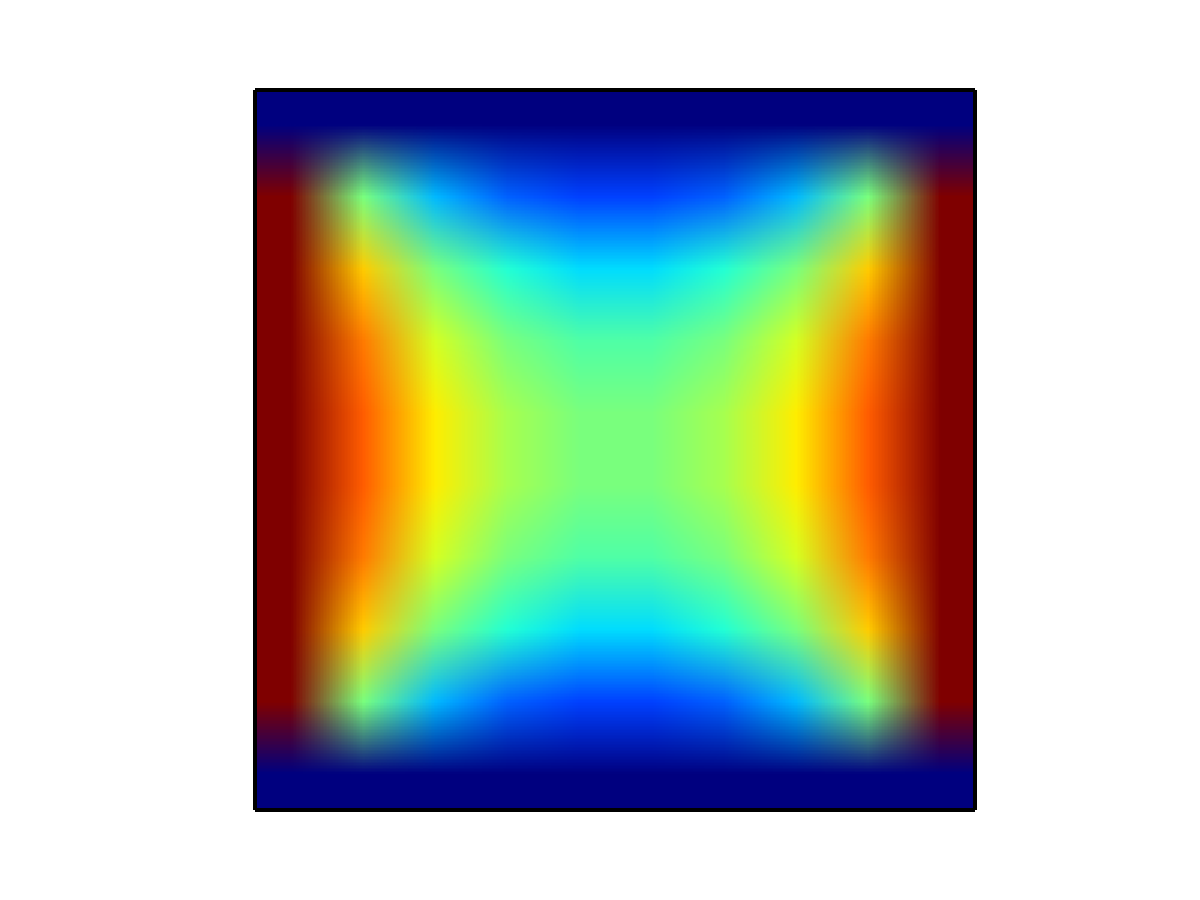
\includegraphics[width=\linewidth]{jacobi_small.pdf}
    \caption{$10\times 10$ approximation.}
\end{subfigure}%
\begin{subfigure}{.5\textwidth}
    \centering
    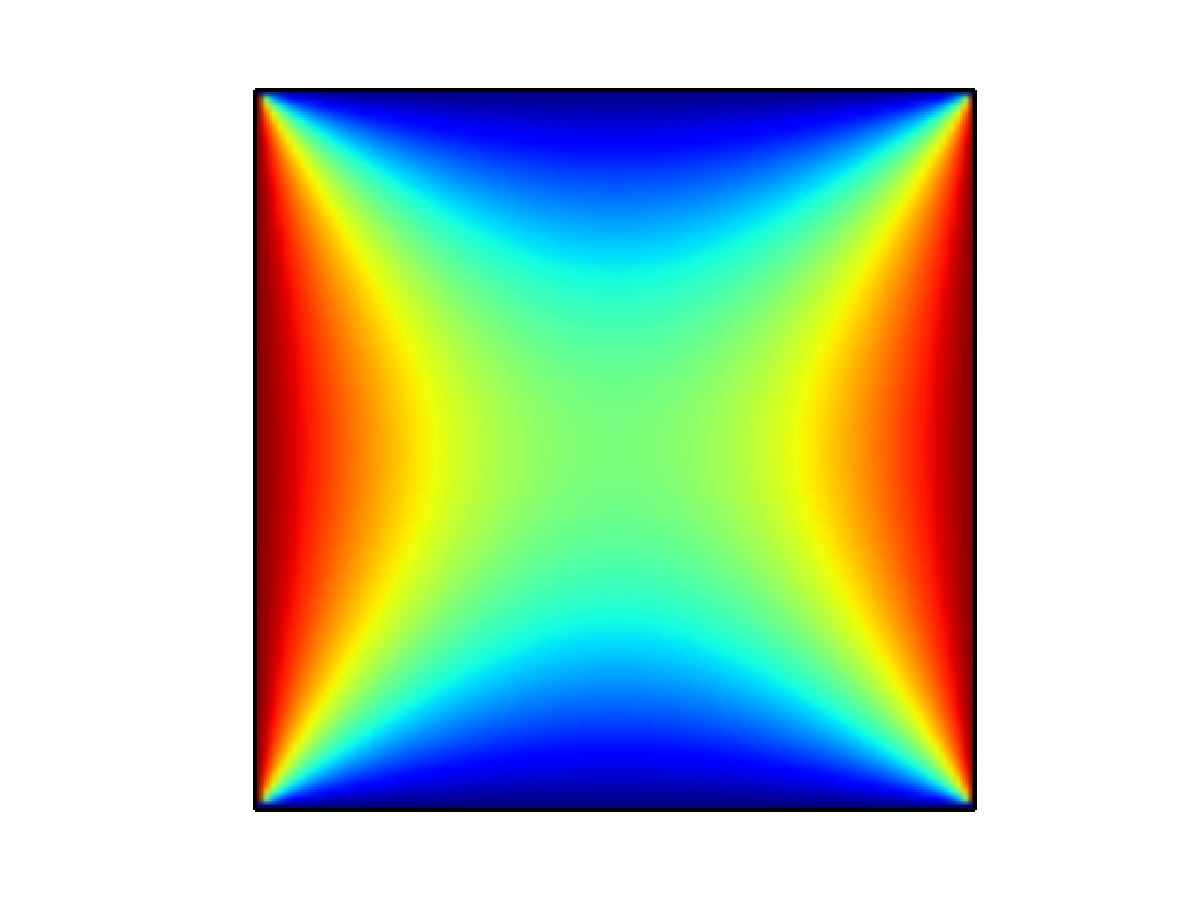
\includegraphics[width=\linewidth]{jacobi_big.pdf}
    \caption{$100\times 100$ approximation.}
\end{subfigure}
\caption{Hot plates in steady state with different resolutions.}
\end{figure}
\end{comment} % Move to Iterative Methods ^^^^^^^^^^^^^^^^^^^^^^^^^^^^^^^^^^^^^
